\documentclass[10pt]{article}

\usepackage[T1]{fontenc}
\usepackage[utf8]{inputenc}
%\usepackage{beton}
%\usepackage{ccfonts}
%\usepackage{concrete}
\usepackage{concmath}
\usepackage{eulervm}
\usepackage{amsmath,amsthm,amssymb}
\usepackage{mathtools}
\usepackage{multicol}
\usepackage{marginnote}
\usepackage{pgfplots}
\usepackage{float}
\usepackage{hyperref}
\pgfplotsset{compat=1.5}

\usepackage{mathtools}

\usepackage{wasysym}
\usepackage[margin=1.5in]{geometry} 
\usepackage{enumerate}
\index{\usepackage}\usepackage{multicol}

\newcommand{\N}{\mathbf{N}}
\newcommand{\Z}{\mathbb{Z}}

\newcommand{\R}{\mathbf{R}}
\newcommand{\C}{\mathbf{C}}
\newcommand{\Pbb}{\mathbb{P}}
\newcommand{\Fcal}{\mathcal{F}}
\newcommand{\Acal}{\mathcal{A}}
\newcommand{\Ecal}{\mathcal{E}}
\newcommand{\Ebb}{\mathbb{E}}
\newcommand{\Qbb}{\mathbb{Q}}

\newenvironment{theorem}[2][Theorem]{\begin{trivlist}
  \item[\hskip \labelsep {\bfseries #1}\hskip \labelsep {\bfseries #2.}]}{\end{trivlist}}
\newenvironment{lemma}[2][Lemma]{\begin{trivlist}
  \item[\hskip \labelsep {\bfseries #1}\hskip \labelsep {\bfseries #2.}]}{\end{trivlist}}
\newenvironment{exercise}[2][Exercise]{\begin{trivlist}
  \item[\hskip \labelsep {\bfseries #1}\hskip \labelsep {\bfseries #2.}]}{\end{trivlist}}
\newenvironment{reflection}[2][Reflection]{\begin{trivlist}
  \item[\hskip \labelsep {\bfseries #1}\hskip \labelsep {\bfseries #2.}]}{\end{trivlist}}
\newenvironment{proposition}[2][Proposition]{\begin{trivlist}
  \item[\hskip \labelsep {\bfseries #1}\hskip \labelsep {\bfseries #2.}]}{\end{trivlist}}
\newenvironment{corollary}[2][Corollary]{\begin{trivlist}
  \item[\hskip \labelsep {\bfseries #1}\hskip \labelsep {\bfseries #2.}]}{\end{trivlist}}

\newenvironment{definition}[2][Definition]{\begin{trivlist}
  \item[\hskip \labelsep {\bfseries #1}\hskip \labelsep {\bfseries #2.}]}{\end{trivlist}}

\begin{document}
	
  \renewcommand{\qedsymbol}{\smiley}
	\title{Investments Class \\ Problem set 1}
	\author{Daniel Grosu, William Martin, Denis Steffen}
	
	\maketitle

  \begin{exercise}{1}
    First, we need to solve the Geometric Brownian Motion SDE. 
    The SDE is given by: 
    $$ \frac{dS_t}{S_t} = \mu dt + \sigma dz_t$$ where $z_t$ is a standard Brownian Motion. 
    We can apply Itô's lemma on the stochastic process $Y_t = f(S_t) = \ln(S_t)$.
    Thus, $$ dY_t = 0 dt +  \frac{1}{S_t}dS_t + \frac{1}{2}\frac{-1}{S_t^2}(\sigma S_t)^2 dt = \mu dt + \sigma dz_t - \frac{\sigma^2}{2}dt$$
    and $$ \ln(S_t) = (\mu-\frac{\sigma^2}{2})t + \sigma dz_t$$
    The solution of the SDE is: $ S_t = S_0 \exp((\mu-\frac{\sigma^2}{2})t+ \sigma z_t)$.
    Simulating on $10$ years, with the given drift and volatility parameters, the share price can be found in Figure \ref{GMB}. The corresponding log-returns of the share are displayed in Figure \ref{DLR}.
    With this data, we can compute the annualized mean and standard deviation of log-returns:
    
    \begin{table}[H]
      \centering
        \begin{tabular}{|l|l|}
        \hline
        Annualized mean & Annualized Standard Deviation \\ \hline
        7.659 \%        & 20.336 \%                    \\ \hline
        \end{tabular}
        \caption{Simulation log-returns statistics}
      \end{table}
      We can see that the estimators of simulated share prices are consistent with the parameters $\mu = 6\%$ and $\sigma = 20\%$ but there is still high variance in the estimation. 

  \begin{figure}[H]
	\centering
	\begin{minipage}[b]{0.49\textwidth}
		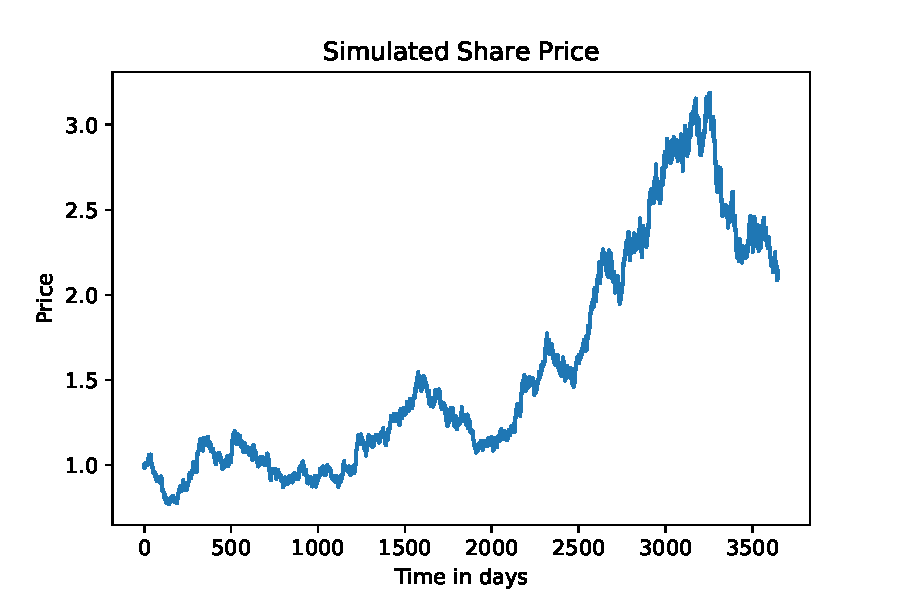
\includegraphics[width = \textwidth]{Figures/simulation.pdf}
		\caption{Share price simulation}
		\label{GMB}
	\end{minipage}
	\hfill
	\begin{minipage}[b]{0.49\textwidth}
		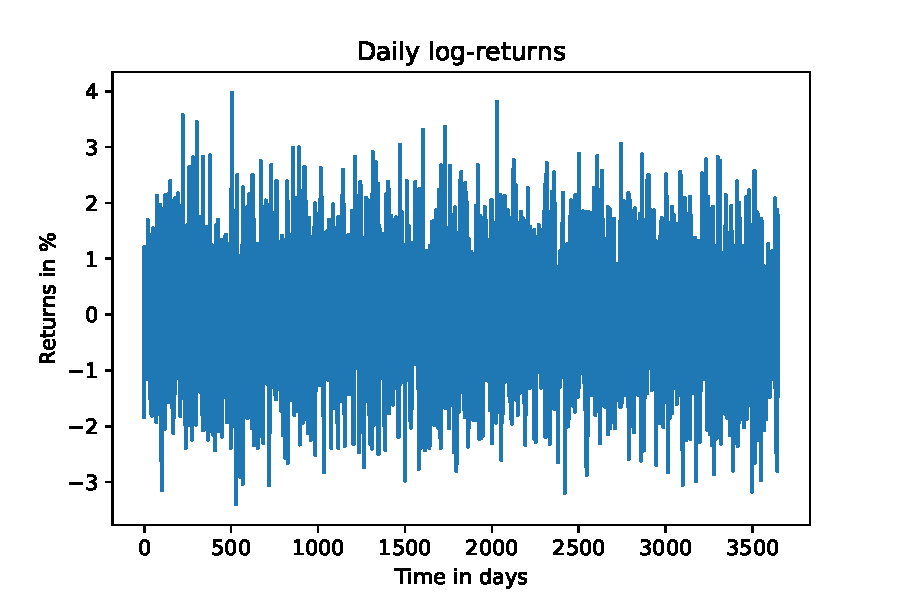
\includegraphics[width = \textwidth]{Figures/logreturns.pdf}
		\caption{Daily log-returns}
		\label{DLR}
  \end{minipage}	
  \end{figure}
  \end{exercise}

	\newpage

  \begin{exercise}{2}
    To control the accuracy of our estimators of the mean and the volatility, we can simulate more samples and estimate the variance of these two estimators.
    We have simulated daily share prices from January $1^{\text{st}}$, $1950$ to December $31^{\text{st}}$, 2018 and so we get $25202$ daily samples. We can resample the daily prices into monthly ones by taking local monthly averages. The graph of the daily and averaged monthly share prices are in Figures \ref{GMB2} and \ref{GMB2M}.
    \begin{figure}[H]
      \centering
      \begin{minipage}[b]{0.49\textwidth}
        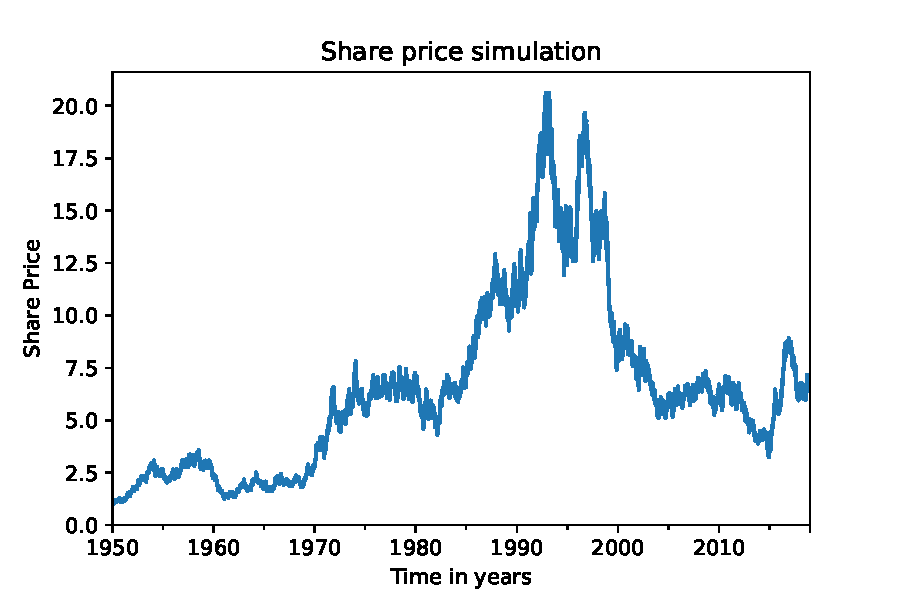
\includegraphics[width = \textwidth]{Figures/simulation2.pdf}
        \caption{Share price simulation (daily)}
        \label{GMB2}
      \end{minipage}
      \hfill
      \begin{minipage}[b]{0.49\textwidth}
        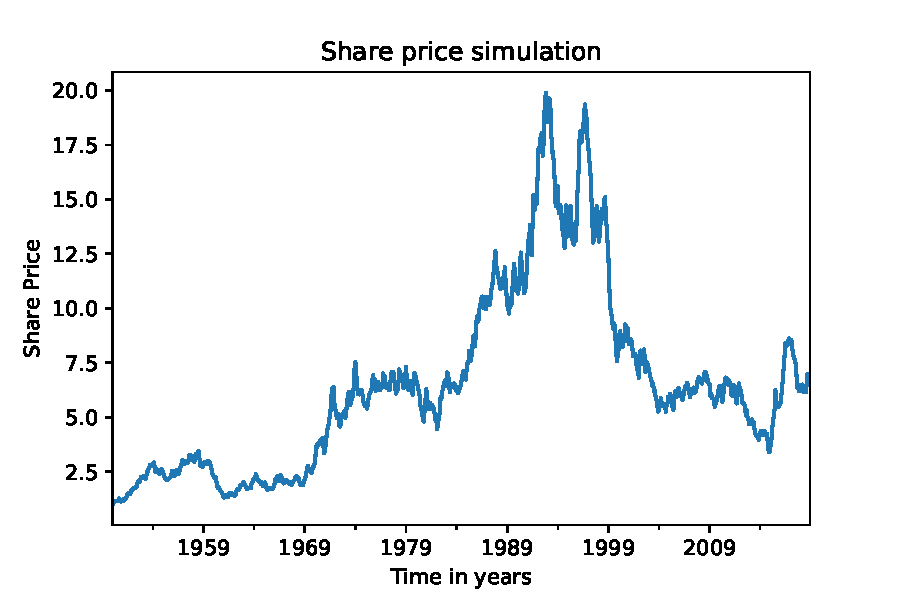
\includegraphics[width = \textwidth]{Figures/simulation2monthly.pdf}
        \caption{Monthly average}
        \label{GMB2M}
      \end{minipage}	
      \end{figure}
  \end{exercise}
  
	\newpage  
  
  \begin{exercise}{3}
 	 
	From our simulated data of daily prices, we generate time-series of daily, weekly, and monthly log-returns and compute a summary statistics for each frequency (using the \textit{describe()} method from the \textit{pandas} library) :
	
	\bigbreak
	
	\begin{tabular}{ |p{3cm}||p{3cm}|p{3cm}|p{3cm}|  }
 		\hline
		\multicolumn{4}{|c|}{Summary statistics of log returns} \\
		\hline
		Data & Daily & Weekly & Monthly\\
 		\hline
 		count   &  25201 & 3601 & 827\\
 		mean & 0.000116 & 0.000812 & 0.003565\\
 		std & 0.010416 & 0.027782 & 0.057413\\
 		min & -0.041882 & -0.099737 & -0.177405\\
 		25\% &  -0.006899 & -0.017644 & -0.033800\\
 		50\% & 0.000300 & 0.000883 & 0.003040\\
 		75\% & 0.007208 & 0.019693 & 0.041604\\
 		max & 0.042026 & 0.107188 & 0.172747\\
 		\hline
	\end{tabular}

	\bigbreak	
	
	For each frequency, we then proceed to compute the annualized mean and standard deviation of the log-returns: 
	
	\bigbreak
	
	\begin{tabular}{ |p{3cm}||p{3cm}|p{3cm}|p{3cm}|  }
		\hline
	 	\multicolumn{4}{|c|}{Annualized metrics of log-returns} \\
	 	\hline
	 	Data & Daily & Weekly & Monthly\\
 		\hline
 		mean  &  0.042358 & 0.042232 & 0.042778\\
 		std & 0.198990 & 0.200312 & 0.198765\\
 		\hline
	\end{tabular}
	
	\bigbreak	
	
	Using a rolling one-year window, we plot the time-series of the annualized mean and std deviation of log-returns estimates for each frequency:
	
	\begin{figure}[H]
	
		\centering
		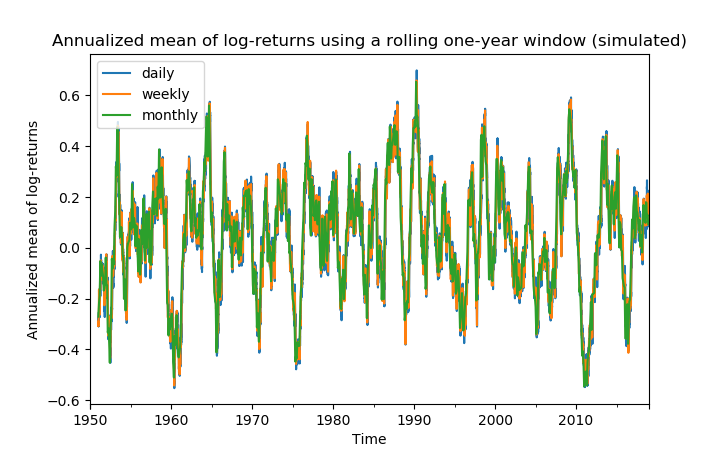
\includegraphics[scale=0.5]{Figures/problem3d_mean.png}	
		\caption{Annualized mean of log-returns of simulated data (daily, weekly, monthly)}	
		\label{fig:problem3d_mean}
	
	\end{figure}
	
	\begin{figure}[H]
	
		\centering
		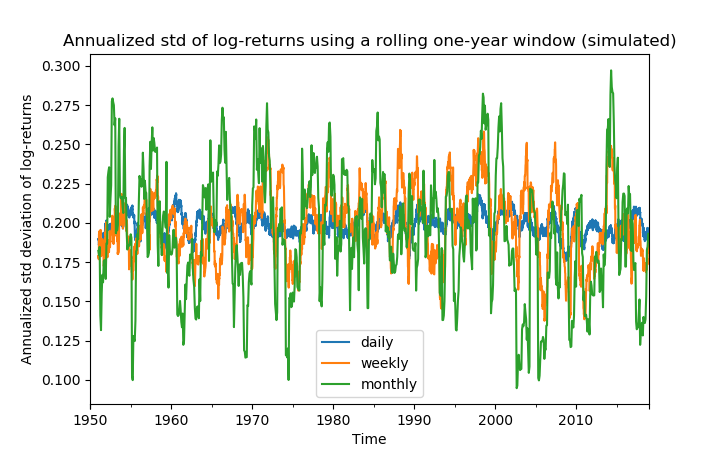
\includegraphics[scale=0.5]{Figures/problem3d_std.png}	
		\caption{Annualized std deviation of log-returns of simulated data (daily, weekly, monthly)}	
		\label{fig:problem3d_std}
	
	\end{figure}
	
	From Figure \ref{fig:problem3d_mean}, we observe that the estimation of the annualized mean of log-returns using a rolling one-year window is very noisy. As a matter of fact, the estimation varies from approximately +/- 60\% where in reality it is 6\% for all frequencies. Thus, varying the frequency does not improve the estimation of the mean but increasing the horizon length  will. 
	
	\smallbreak
	
	From Figure \ref{fig:problem3d_std}, we observe that increasing the frequency (from monthly to daily) improves the estimation of the standard deviation quite considerably. Indeed, at a monthly frequency, we observe estimations of the std deviation varying from 10\% to 30\% approximately where in reality it is 20\%. At a daily frequency, the estimates vary closely around the real value. In conclusion, increasing the frequency allows us to better estimate the volatility. 
  
	\bigbreak
	
	 We recall that the estimator of $\mu$ is given by the sample mean:
	 
	\begin{align*}
		\hat{\mu} = \frac{1}{n \Delta}\sum^{n}_{i = 1}R_{i}
	\end{align*}
	
	And that the simple estimator of the variance is computed as follows (which does not depend on $\hat{\mu}$):
	
	\begin{align*}
		\hat{\sigma^{2}} = \frac{1}{n \Delta}\sum^{n}_{i = 1}(R_{i})^{2}
	\end{align*}
	 
	 For daily and monthly frequencies, we compute the mean and variance of both our mean and variance estimator, as well as the theoretical values:
	 
	 \bigbreak
	 
	 \begin{tabular}{ |p{3cm}||p{3cm}|p{3cm}|p{3cm}| }
		\hline
	 	\multicolumn{4}{|c|}{Metrics of mean estimator} \\
	 	\hline
	 	Data & Daily & Monthly & Theoretical\\
 		\hline
 		mean  &  0.042348 & 0.042354 & 0.06 \\
 		variance & 0.043211 & 0.043283 & 0.04\\
 		\hline
	\end{tabular}
	
	\bigbreak	
	
	\begin{tabular}{ |p{2cm}||p{2cm}|p{3cm}|p{2cm}|p{3cm}| }
		\hline
	 	\multicolumn{5}{|c|}{Metrics of variance estimator} \\
	 	\hline
	 	Data & Daily & Theoretical daily  & Monthly & Theoretical monthly \\
 		\hline
 		mean  &  0.039602 & 0.040009 & 0.039660 & 0.040300\\
 		variance & 7.274037e-06 & 8.771446e-06 & 0.000178 & 0.000270 \\
 		\hline
	\end{tabular}
	
	\bigbreak

	Where we have taken the formulae for theoretical values for the mean and variance of both the mean and variance estimators:
	
	\begin{align*}
		\Ebb[\hat{\mu}] = \mu \\
		Var[\hat{\mu}] = \frac{\sigma^{2}}{T} \\
		\Ebb[\hat{\sigma}^{2}] = \sigma^{2} + \mu^{2} \frac{T}{n} \\
		Var[\hat{\sigma}^{2}] = \frac{2\sigma^{4}}{n} + 4\mu^{2}\sigma^{2}\frac{T}{n^{2}}
	\end{align*}
	
	The first moments of the sample mean are not too far off of their theoretical counterparts although we know from the course that the sample mean is an unbiased estimator of $\mu$.
	
	\smallbreak
	
	Finally, we saw in the course that the estimator of the variance is biased but we see that even with a monthly frequency, the estimation is pretty accurate. For both frequencies, we see that the variance estimator is reduced to 0.
  
  \end{exercise}

	\newpage
	
  \begin{exercise}{4}
  
	We proceed similarly as in exercise 3 but with real data.
	
	\bigbreak	
		
	\textbf{Apple}
	
	\smallbreak
	
	The summary statistics are the followings:
	
	\bigbreak	
	
	\begin{tabular}{ |p{3cm}||p{3cm}|p{3cm}|p{3cm}|  }
 		\hline
		\multicolumn{4}{|c|}{Summary statistics of log returns of Apple} \\
		\hline
		Data & Daily & Weekly & Monthly\\
 		\hline
 		count   &  4527 & 940 & 216\\
 		mean & 0.001132 & 0.005518 & 0.023517\\
 		std & 0.023080 & 0.049161 & 0.105660\\
 		min & -0.197470 & -0.290710 & -0.453292\\
 		25\% & -0.010026 & -0.022411 & -0.027271\\
 		50\% & 0.000860 & 0.008078 & 0.030809\\
 		75\% & 0.012450 & 0.034924 & 0.089654\\
 		max & 0.130194 & 0.220095 & 0.337724\\
 		\hline
	\end{tabular}
	
	\bigbreak	
	
	For each frequency, we then proceed to compute the annualized mean and standard deviation of the log-returns:
	
	\bigbreak
	
	\begin{tabular}{ |p{3cm}||p{3cm}|p{3cm}|p{3cm}|  }
		\hline
	 	\multicolumn{4}{|c|}{Annualized metrics of log-returns of Apple} \\
	 	\hline
	 	Data & Daily & Weekly & Monthly\\
 		\hline
 		mean  &  0.285267 & 0.286937 & 0.282208\\
 		std & 0.366347 & 0.354317 & 0.365167\\
 		\hline
	\end{tabular}
	
	\bigbreak	
	
	Using a rolling one-year window, we plot the time-series of the annualized mean and std deviation of log-returns estimates for each frequency:
	
	\begin{figure}[H]
	
		\centering
		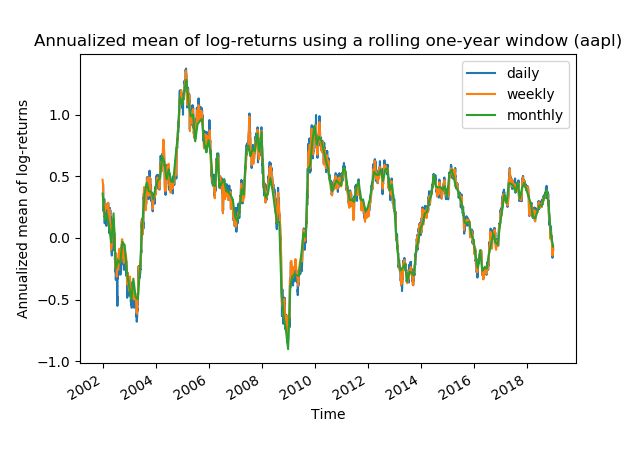
\includegraphics[scale=0.5]{Figures/problem4d_mean_aapl.png}	
		\caption{Annualized mean of log-returns of Apple (daily, weekly, monthly)}	
		\label{fig:problem3d_mean_aapl}
	
	\end{figure}
	
	\begin{figure}[H]
	
		\centering
		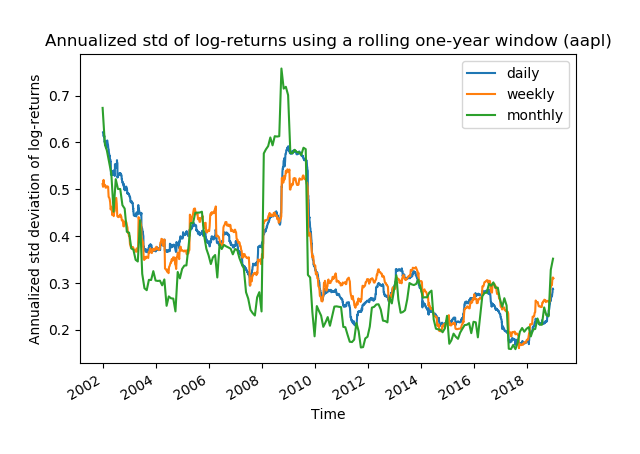
\includegraphics[scale=0.5]{Figures/problem4d_std_aapl.png}	
		\caption{Annualized std deviation of log-returns of Apple (daily, weekly, monthly)}	
		\label{fig:problem3d_std_aapl}
	
	\end{figure}
		
	\bigbreak	
		
	\textbf{Goldman Sachs}
	
	\smallbreak
	
	The summary statistics are the followings:
	
	\bigbreak	
	
	\begin{tabular}{ |p{3cm}||p{3cm}|p{3cm}|p{3cm}|  }
 		\hline
		\multicolumn{4}{|c|}{Summary statistics of log returns of Goldman Sachs} \\
		\hline
		Data & Daily & Weekly & Monthly\\
 		\hline
 		count   &  4527 & 940 & 216\\
 		mean & 0.000141 & 0.000766 & 0.004757\\
 		std & 0.022295 & 0.047307 & 0.083148\\
 		min & -0.210223 & -0.427937 & -0.290885\\
 		25\% & -0.009903 & -0.022032 & -0.050073\\
 		50\% & 0.000244 & 0.003461 & 0.014704\\
 		75\% & 0.010450 & 0.025272 & 0.056586\\
 		max & 0.234818 & 0.356032 & 0.195242\\
 		\hline
	\end{tabular}
	
	\bigbreak	
	
	For each frequency, we then proceed to compute the annualized mean and standard deviation of the log-returns:
	
	\bigbreak
	
	\begin{tabular}{ |p{3cm}||p{3cm}|p{3cm}|p{3cm}|  }
		\hline
	 	\multicolumn{4}{|c|}{Annualized metrics of log-returns of Goldman Sachs} \\
	 	\hline
	 	Data & Daily & Weekly & Monthly\\
 		\hline
 		mean  &  0.035651 & 0.039821 & 0.057080\\
 		std & 0.353886 & 0.340952 & 0.287366\\
 		\hline
	\end{tabular}
	
	\bigbreak	
	
	Using a rolling one-year window, we plot the time-series of the annualized mean and std deviation of log-returns estimates for each frequency:
	
	\begin{figure}[H]
	
		\centering
		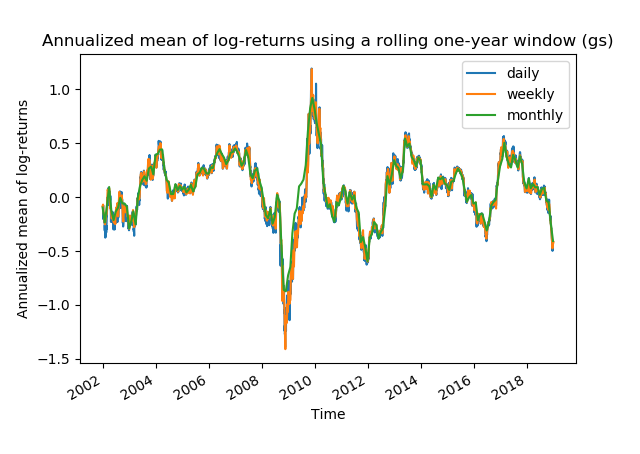
\includegraphics[scale=0.5]{Figures/problem4d_mean_gs.png}	
		\caption{Annualized mean of log-returns of Goldman Sachs (daily, weekly, monthly)}	
		\label{fig:problem3d_mean_gs}
	
	\end{figure}
	
	\begin{figure}[H]
	
		\centering
		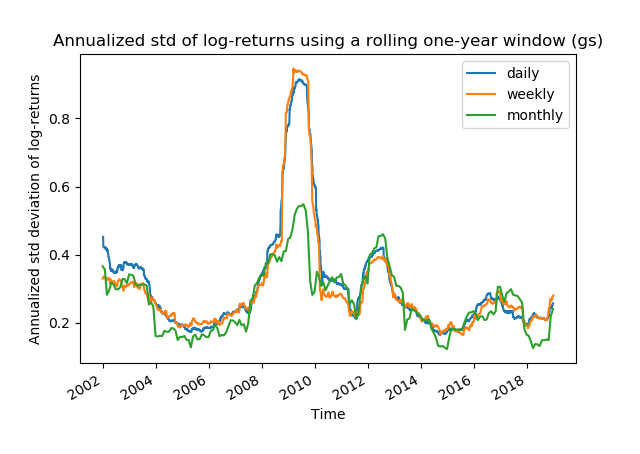
\includegraphics[scale=0.5]{Figures/problem4d_std_gs.png}	
		\caption{Annualized std deviation of log-returns of Goldman Sachs (daily, weekly, monthly)}	
		\label{fig:problem3d_std_gs}
	
	\end{figure}

	\bigbreak	
		
	\textbf{Microsoft}
	
	\smallbreak
	
	The summary statistics are the followings:
	
	\bigbreak	
	
	\begin{tabular}{ |p{3cm}||p{3cm}|p{3cm}|p{3cm}|  }
 		\hline
		\multicolumn{4}{|c|}{Summary statistics of log returns of Microsoft} \\
		\hline
		Data & Daily & Weekly & Monthly\\
 		\hline
 		count   &  4527 & 940 & 216\\
 		mean & 0.000435 & 0.002210 & 0.009887\\
 		std & 0.017863 & 0.036112 & 0.070669\\
 		min & -0.124578 & -0.219669 & -0.189425\\
 		25\% & -0.007842 & -0.016186 & -0.035620\\
 		50\% & 0.000271 & 0.002047 & 0.018235\\
 		75\% & 0.008638 & 0.021435 & 0.051449\\
 		max & 0.170626 & 0.143311 & 0.306621\\
 		\hline
	\end{tabular}
	
	\bigbreak	
	
	For each frequency, we then proceed to compute the annualized mean and standard deviation of the log-returns:
	
	\bigbreak
	
	\begin{tabular}{ |p{3cm}||p{3cm}|p{3cm}|p{3cm}|  }
		\hline
	 	\multicolumn{4}{|c|}{Annualized metrics of log-returns of Microsoft} \\
	 	\hline
	 	Data & Daily & Weekly & Monthly\\
 		\hline
 		mean  &  0.109558 & 0.114940 & 0.118649\\
 		std & 0.283531 & 0.260270 & 0.244236\\
 		\hline
	\end{tabular}
	
	\bigbreak	
	
	Using a rolling one-year window, we plot the time-series of the annualized mean and std deviation of log-returns estimates for each frequency:
	
	\begin{figure}[H]
	
		\centering
		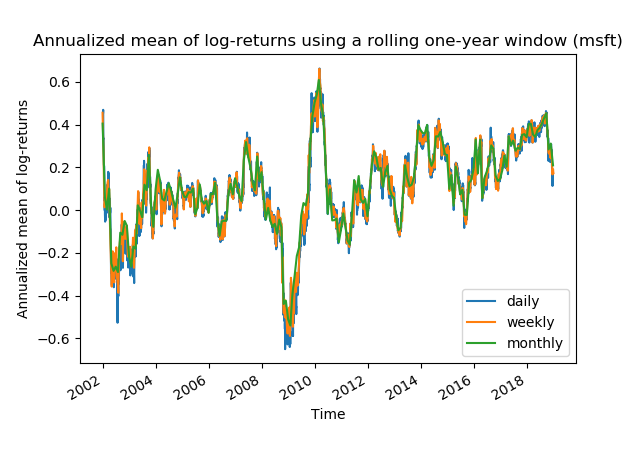
\includegraphics[scale=0.5]{Figures/problem4d_mean_msft.png}	
		\caption{Annualized mean of log-returns of Microsoft (daily, weekly, monthly)}	
		\label{fig:problem3d_mean_msft}
	
	\end{figure}
	
	\begin{figure}[H]
	
		\centering
		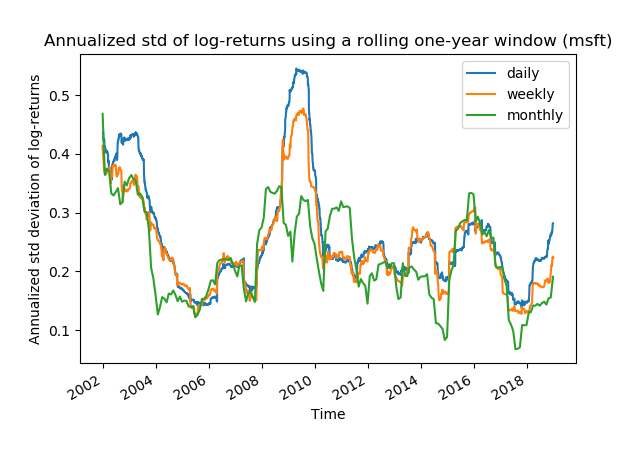
\includegraphics[scale=0.5]{Figures/problem4d_std_msft.png}	
		\caption{Annualized std deviation of log-returns of Microsoft (daily, weekly, monthly)}	
		\label{fig:problem3d_std_msft}
	
	\end{figure}	  
  
	\bigbreak	
		
	\textbf{Procter and Gamble}
	
	\smallbreak
	
	The summary statistics are the followings:
	
	\bigbreak	
	
	\begin{tabular}{ |p{3cm}||p{3cm}|p{3cm}|p{3cm}|  }
 		\hline
		\multicolumn{4}{|c|}{Summary statistics of log returns of Procter and Gamble} \\
		\hline
		Data & Daily & Weekly & Monthly\\
 		\hline
 		count   &  4527 & 940 & 216\\
 		mean & 0.000297 & 0.001451 & 0.006634\\
 		std & 0.011272 & 0.023812 & 0.042314\\
 		min & -0.083161 & -0.187835 & -0.128388\\
 		25\% & -0.004988 & -0.010057 & -0.018551\\
 		50\% & 0.000300 & 0.002197 & 0.009741\\
 		75\% & 0.005703 & 0.014371 & 0.032006\\
 		max & 0.097257 & 0.118140 & 0.108149\\
 		\hline
	\end{tabular}
	
	\bigbreak	
	
	For each frequency, we then proceed to compute the annualized mean and standard deviation of the log-returns:
	
	\bigbreak
	
	\begin{tabular}{ |p{3cm}||p{3cm}|p{3cm}|p{3cm}|  }
		\hline
	 	\multicolumn{4}{|c|}{Annualized metrics of log-returns of Procter and Gamble} \\
	 	\hline
	 	Data & Daily & Weekly & Monthly\\
 		\hline
 		mean  &  0.074738 & 0.075452 & 0.079604\\
 		std & 0.178924 & 0.171622 & 0.146239\\
 		\hline
	\end{tabular}
	
	\bigbreak	
	
	Using a rolling one-year window, we plot the time-series of the annualized mean and std deviation of log-returns estimates for each frequency:
	
	\begin{figure}[H]
	
		\centering
		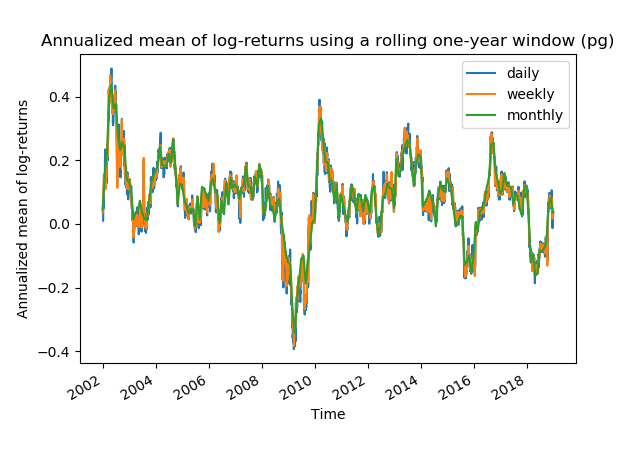
\includegraphics[scale=0.5]{Figures/problem4d_mean_pg.png}	
		\caption{Annualized mean of log-returns of Procter and Gamble (daily, weekly, monthly)}	
		\label{fig:problem3d_mean_pg}
	
	\end{figure}
	
	\begin{figure}[H]
	
		\centering
		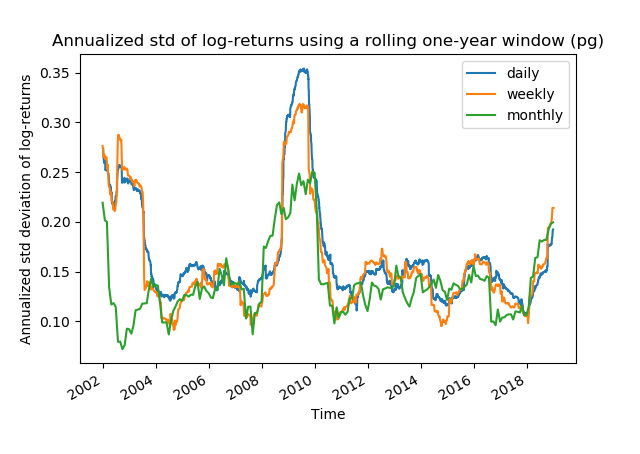
\includegraphics[scale=0.5]{Figures/problem4d_std_pg.png}	
		\caption{Annualized std deviation of log-returns of Procter and Gamble (daily, weekly, monthly)}	
		\label{fig:problem3d_std_pg}
	
	\end{figure}	  
 
	\bigbreak	
		
	\textbf{General Electric}
	
	\smallbreak
	
	The summary statistics are the followings:
	
	\bigbreak	
	
	\begin{tabular}{ |p{3cm}||p{3cm}|p{3cm}|p{3cm}|  }
 		\hline
		\multicolumn{4}{|c|}{Summary statistics of log returns of General Electric} \\
		\hline
		Data & Daily & Weekly & Monthly\\
 		\hline
 		count   &  4527 & 940 & 216\\
 		mean & -0.000282 & -0.001314 & -0.005171\\
 		std & 0.019175 & 0.041075 & 0.079993\\
 		min & -0.136841 & -0.246562 & -0.356068\\
 		25\% &  -0.008103 & -0.018518 & -0.044020\\
 		50\% & 0.000000 & -0.000495 & -0.003015\\
 		75\% & 0.007908 & 0.018517 & 0.040110\\
 		max & 0.179844 & 0.289828 & 0.214621\\
 		\hline
	\end{tabular}
	
	\bigbreak	
	
	For each frequency, we then proceed to compute the annualized mean and standard deviation of the log-returns:
	
	\bigbreak
	
	\begin{tabular}{ |p{3cm}||p{3cm}|p{3cm}|p{3cm}|  }
		\hline
	 	\multicolumn{4}{|c|}{Annualized metrics of log-returns of General Electric} \\
	 	\hline
	 	Data & Daily & Weekly & Monthly\\
 		\hline
 		mean  &  -0.071126 & -0.068346 & -0.062046\\
 		std & 0.304355 & 0.296039 & 0.276460\\
 		\hline
	\end{tabular}
	
	\bigbreak	
	
	Using a rolling one-year window, we plot the time-series of the annualized mean and std deviation of log-returns estimates for each frequency:
	
	\begin{figure}[H]
	
		\centering
		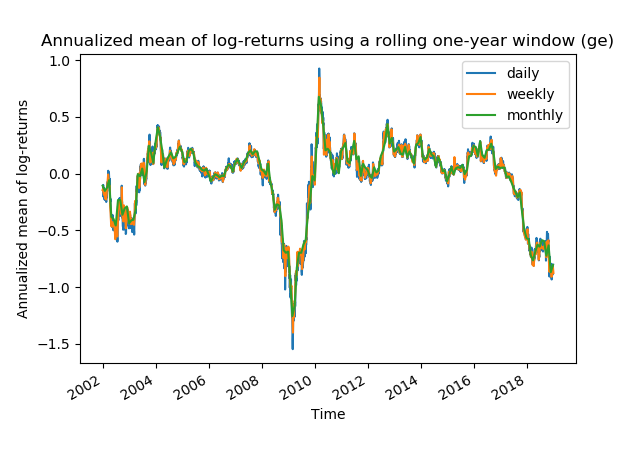
\includegraphics[scale=0.5]{Figures/problem4d_mean_ge.png}	
		\caption{Annualized mean of log-returns of General Electric (daily, weekly, monthly)}	
		\label{fig:problem3d_men_ge}
	
	\end{figure}
	
	\begin{figure}[H]
	
		\centering
		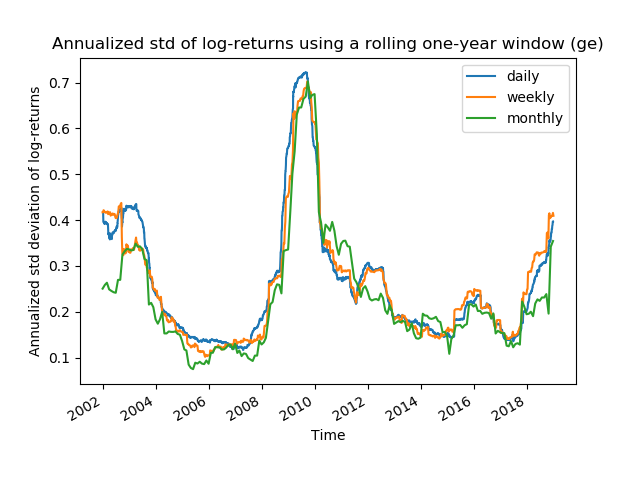
\includegraphics[scale=0.5]{Figures/problem4d_std_ge.png}	
		\caption{Annualized std deviation of log-returns of General Electric (daily, weekly, monthly)}	
		\label{fig:problem3d_std_ge}
	
	\end{figure} 
	
	The variation of the time-series of the annualized mean using a rolling one-year window on real data seems to be larger than with simulated data. Indeed, we observe variations around $+/- 60\%$ in exercise 3, whereas with real data, this variations often go beyond this interval. This makes the job of estimating the expected return on stocks more difficult.  
 
	\smallbreak
	
	For the time-series of the annualized standard deviation of a rolling one-year window, we observe a very big difference between real and simulated data. With simulated data, our conclusion were that by increasing the frequency, we were able to improve the estimation of the standard deviation by quite a margin. This is not at all the case now with real data. On the contrary, the range of the time-series remains large even at high frequencies. This can be explained by the fact that we assumed a constant volatility whereas in real life, the volatility varies over time, making the job of estimating quite difficult. 
 
  \end{exercise} 

  %\section*{Python Code}

  % \subsection*{Exercise}
  % \lstinputlisting{code/exercise.py}
\end{document}

